\chapter{Related work}
Now we present a comprehensive analysis of related literature about three main topics: developers' activities, work fragmentation and mining software repositories. All these topics belong to software engineering research and they close each other; some of the cited literature are a convergence of multiple subjects. We start by describing research about developers' activities.

\section{Developers' activities}
In recent years there has been a lot of effort in understanding the way developers work and the challenges they face. With that information we can design tools \cite{CD10, P14, CLQ15, KM06} that offer better conditions on everyday activities. 

Singel et al. \cite{SLV10} surveyed developers to get information of common work practices. They found that programmers spend about half of the time writing code and attending to meetings, and a third or less of the time doing research, configuring, fixing bugs, designing and testing. When shadowing software engineers they were able to get several categories for the activities performed: call trace, consult, compile, configuration, debug, documentation, edit, management, in-house tools, notes, search, source, hardware and UNIX. From these activities, search, looking at the source and editing are the most common in the group of programmers involved in the study. Similarly, LaToza et al. \cite{LVD06} defined a category of activities related to code and motivation: designing, writing, understanding, editing, unit testing, communicating, overhead, other code and non code. The difference between both classifications is that the latter considers collaboration activities with other developers.

Murphy et al. \cite{MKF06} analyzed usage data of multiple programmers with the Eclipse IDE. They found that some of the most commonly executed commands are delete, save, next word and paste. Also, they found that programmers use 11 kinds of refactoring commands (e.g. rename, move, extract and pull up); these commands are often executed via key bindings and exploring the menus.

Program understanding (referred also as program comprehension) involves all kinds of activities meant to better understand the code in development, such as reading the code and documentation, follow a problem-solution-test pattern, interacting with the UI (User Interface), debugging the application, taking notes and more techniques according to Roehm et al. \cite{RTK12}. According to Rugaber \cite{R95}, the difficulty of program comprehension lies in its objective of bridging different concepts, including application domain and solution, the program and the abstraction of design descriptions, and the hierarchical world of programs and the associational nature of human cognition. It is an activity that covers a considerable working time of a developer. There are many studies with estimations of the magnitude of this activity; Fjeldstad and Hamlen \cite{FH83} estimate that about half of the time of software maintaining tasks are spent in program comprehension; Beller et al. \cite{BGZ15} observed that programmers spent 70\% reading code rather than writing, agreeing with Baracchi \cite{B14} on this proportion; Minelli et al. \cite{MMLK14} analyzed usage data and concluded that program comprehension can account from 54\% to 90\% of a working session.

Baracchi \cite{B14} analyzed four kinds of programmer's activities: understanding, editing, inspection and navigation. His findings indicate that the edition activities can be only 20\% of a working session and understanding more than 70\%. Moreover, he classified the working sessions in four groups: Enhancement, Bug-fixing, Refactoring and General. Enhancement sessions are the most common and are followed by the General purpose type of sessions. He uses interaction data with the IDE (Integrated Development Environment).

About testing tasks, Beller et al. \cite{BGZ15} developed a tool to extract usage data from the IDE in order to study the testing practices of software developers. They found that on average they spent 9\% the time testing code, but it can get well below that percentage. Also, developers execute about 5 tests per day roughly every 50 minutes.


On refactoring activities, Murphy-Hill et al. \cite{MPB12} used the Eclipse Usage Data Collector dataset to understand how programmers are using refactoring tools analyzing the patterns of refactoring practices, finding that most programmers do not make deep use of these tools, leaving untouched most of the configuration parameters and performing manually most of the refactoring.

\section{Work Fragmentation}
Work Fragmentation is defined as a break of the work in progress and it is a pervasive phenomenon in all sorts of workers, such as information workers, a group in which developers belong. The activities of an information worker are characterized by spending short time in one task and switching to others frequently \cite{MGH05}. A fragmented working time is constantly interrupted and the frequency depends on the nature of the business \cite{T99}. Some examples of interruptions are emails \cite{BJE05}, notifications \cite{CCH01}, coworkers \cite{LVD06}, meetings \cite{LR05} and oneself \cite{MGH05}.

Mark et al. \cite{MGH05} indicate that interruptions are a common affection of information workers (e.g. administrators, developers and financial analysts). In a field study in an information technology company they found that around 57\% of the working spheres (a day of work is composed of multiple working spheres) are interrupted, and these spheres last only 11 minutes (in average) before going to another sphere or giving place to an interruption. Also, they identified external interruptions (e.g. environment events) and internal interruptions (e.g. taking a break or looking for the solution to a problem). In programmers and analysts the internal and external interruptions occur at the same proportion.

Similar to the previously cited work, much of the research done about interruptions is trough observational studies, experiments and surveys to a broad range of workers. Eyrolle and Cellier \cite{EC00} implemented a laboratory study with telecommunications operators and found that the processing time of a task increases in the presence of interruptions as well as the rate of errors within the first 30 seconds after starting a second task. Bailey et al. \cite{BKC01} also observed a delay on the time spent on a task (subtracting the time spent in interruptions) after having interruptions, and overall a negative effect whose gravity depends on the mental load. They also indicate that interruptions induce annoyance and increase the anxiety and the perceived task difficulty. Burmistrov and Leonova \cite{BL96} executed an exploratory experimental study to measure the impact of interruptions and their complexity on task performance, agreeing with the previous authors that the presence of interruptions increases the time spent on task but also the complexity of the interruption has a significant impact. Cades et al. \cite{CDT07} did an experiment about the complexity or difficulty of interruptions and concluded that more difficult interruptions will lead to greater disruptions, hence increasing the time spent recovering.

Altmann and Trafton \cite{AT04} also found a negative effect of interruptions during an experiment with students performing complex tasks; they attribute the negative effect to the need of recovery called resumption lag, a time invested in the recovery from an interruption. They conclude that having cues available during the resumption lag helps to decrease the time invested in this phase. Iqbal and Horvitz \cite{IH07} mention that resuming a task after an interruption can take from a few seconds to several minutes, depending on the kind of the interruption (e.g. messaging and emails); they observed that in average the user takes around 5 minutes to respond to an alert, from 9 to 8 minutes are spent in the interruption and 16 minutes recovering from it. They also present an interruption life cycle involving 4 phases: 
\begin{itemize}
	\item Preparation: time between an alert and the suspension of the task.
	\item Diversion: time spent in the interruption.
	\item Resumption: end of the interruption and resumption of the interrupted task.
	\item Pre-interruption: time spent on the activity before the arrival of a new alert.
\end{itemize}
Parnin \cite{PD10} applied a survey to software developers to better understand the impact of interruptions. According to the results, the most common technique to recover after an interruption is reading the code and navigate backwards in the code until recovering the previous work. For some programmers this is not enough they and use tools to find recent changes in the code. Most of them leave notes, physical or electronic, about the progress before the interruption. Moreover, starting to code after the interruption takes between 10 to 15 minutes, a similar observation to the results of Sanchez et al. \cite{SRV15} who performed an analysis of the interruptions and the impact of productivity with interaction data.


\section{Mining Software Repositories}
The core of this work is within the Mining Software Repositories research area, which can be defined as the extraction of information from different artifacts (e.g. source code, control version logs, documentation and bug reports) that are produced throughout the software development cycle \cite{H04}. This term is not alien to data mining, so the intentions are extracting knowledge and discovering patterns in the data using a set of techniques and algorithms for this goal \cite{FPG96}.

The software repositories can be found in different formats \cite{H08}:
\begin{itemize}
	\item \textbf{Historical repositories}, with information obtained throughout the evolution of a project, e.g., bug reports, emails and control version logs.
	\item \textbf{Runtime repositories}, like deployment information, performance reports and application usage data.
	\item \textbf{Code repositories}, which is access to the source code from a version control such as SVN and Git, or online platforms such as SourceForge or Github.
\end{itemize}

Although some of this repositories are used to keep control of changes and procedures, they are rarely used to make decisions. One of the goals of the Mining Software Repositories field is allowing static repositories to be a guide for decision making, for it is possible to discover important information and patterns that can help predict the future performance of the team and the quality of the product in development \cite{H08, ZZW05}. Each stage of the development of software releases data that can be exploited to make timely decisions. Recently, Hassan \cite{HX10} appointed the name of \emph{Software Intelligence} for all the practices involving Mining Software Repositories within companies.

\subsection{Predicting errors}
There are tasks that have a greater impact with these practices. For example, the project administration can make decisions based on facts and tendencies reflected in the data that can be visualized with metrics, or even predict future events like modules prone to errors based on recent activity.

Related to the latter, there is a great effort in using this data for quality assurance. Khomf et al. \cite{KDZ12} analyzed product release data of the Firefox navigator while the developers were migrating from a traditional release scheme to an agile methodology and found that, though there are the same amount of errors, the users tend to identify them early and the failures are fixed quicker.

Error prediction is another example of the interest in quality. The work made by Nagappan et al. \cite{NBZ06} and Finaly et al. \cite{FPC14} are similar approaches for error prediction using complexity metrics, which are measures of the source code (e.g. the number of lines, functions and classes). Both works agree about the difficulty of predicting errors using solely these metrics and in the low precision of the proposed models. Zimmerman and Nagappan \cite{ZN08} obtained better results considering the structure of the system and the relation between classes, creating a network and obtaining metrics from the related graph. The graph was built identifying the code dependencies of the program, where the nodes are classes and the edges the dependencies between them. From the graph they obtained metrics like the number of nodes, the amount of dependencies in relation to a node and the distance to a node. They found that, although the complexity metrics have better correlation with the amount of errors, the graph metrics can predict well with regression models.

Meneely et al. \cite{MWS08} also used networks to predict errors in modules based on product release data, but instead of representing classes as nodes, they represent the programmers that worked on the project and the edges are created when two of them work in the same piece of code. The authors also used graph metrics to train a predictive model, obtaining a precision of 81\%.

\section{Usage data }
Another example of data that can be captured is the usage data (also called interaction data) between the programmer and the development tools \cite{SnipesETALASD}, which is log of the execution of events within the IDE (Integrated Development Environment). The IDE provides tools to execute tasks effectively, such as navigation between classes and methods, continuous compilation, refactoring, automated testing and debugging, all designed to assist the programmers' productivity. The Figure \ref{fig:ide} shows a screenshot of the Eclipse IDE

\begin{figure}[!ht]
	\centering
	
	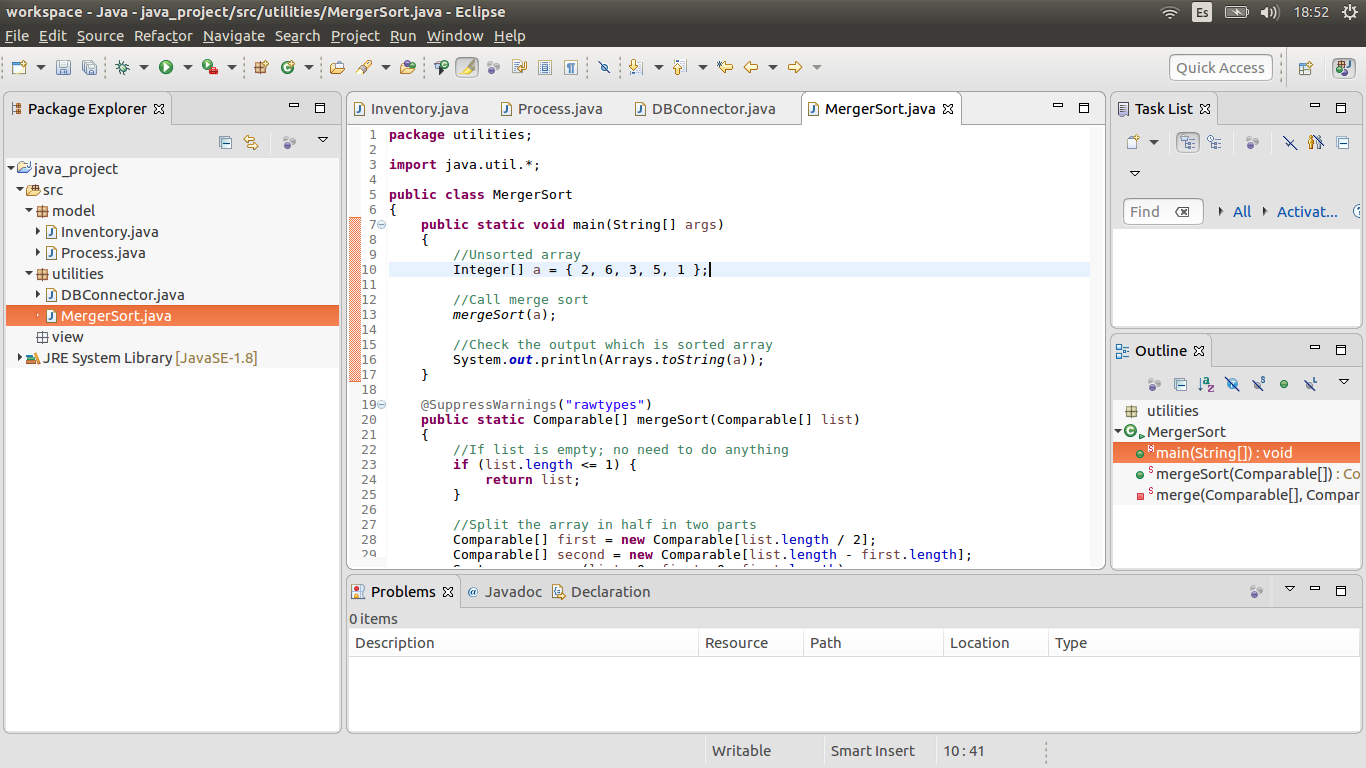
\includegraphics[width=\linewidth,clip=, angle=0]{Figures/IDE}  
	
	\caption{User interface of the Eclipse IDE. }
	\label{fig:ide}
\end{figure}

The usage data is composed of the interactions between the programmer and the IDE, and can include the description of executed commands (e.g. copy, paste, delete and save); the opening or closing of files; clicks, change of line and navigation around text; usage of tools, and more. Generally, everything is stored in a log with date, time and an identifier for the user. As a complement it can contain the name of the class and/or the function where it was executed and the type of the event. The Table \ref{tbl:example_usage_data} shows an fragment of the Eclipse Usage Data Collector dataset with four attributes to represent the user, what kind of command was executed, the description of the command and the date and time of execution.

\begin{changedforreviewerlong}
\begin{table}[ht!]
	\small
	\caption{Example of usage data from the Eclipse Usage Data Collector. }
	\label{tbl:example_usage_data}
	\centering
	\begin{tabular}{p{0.8cm}|p{1.7cm}|p{6.3cm} | p{3cm}} 
		\hline 
		\emph{User} & \emph{Kind} & \emph{Description} & \emph{Datetime}\\  
		\hline 
		\hline 
		5017 & command & org.eclipse.ui.edit.text.goto.lineEnd & 2008-12-15 16:20:28\\
		\hline
		5017 & editor & org.eclipse.wst.jsdt.ui.CompilationUnitEditor & 2008-12-15 16:20:30 \\
		\hline
		5017 & command & org.eclipse.ui.edit.copy & 2008-12-15 16:20:36 \\
		\hline
		5017 & command & org.eclipse.ui.edit.paste & 2008-12-15 16:20:45 \\
		\hline
		5017 & command & org.eclipse.ui.edit.text.goto.lineEnd & 2008-12-15 16:20:46 \\
		\hline
		
	\end{tabular}
\end{table}
\end{changedforreviewerlong}

It is possible to command the IDE to capture usage data to have better understanding, to a low level, of the activities of the programmer \cite{SnipesETALASD}. Eclipse and Visual Studio are examples of IDEs that provide an API (Application Programming Interface) that allows to register all the commands and actions that are begin executed. It is not necessary to build an application to capture the data, for there are several options to collect it like Eclipse Usage Data Collector \cite{MPB12}, Mylyn Monitor \cite{KM06} and Codealike \cite{CLQ15}. It is possible to start a study with existing data from previous projects. An example is the available information in the Eclipse archives about the Usage Data Collector, a dataset of more than 1 million users and 2,000 million registered events.

%\subsection{Productivity metrics}
%Given that the available information about usage data can tell the history of activity of the programmer, one of the most used metrics is the total active time, without the time consumed in interruptions, like the study by Sanchez et al. \cite{SRV15}. The active time is also considered by the focus function of Codealike, which increases when more activity is registered. The focus level is a metric used by this tool to measure the productivity and tries to model the concentration of the user. Prolonged time without registered activity o time outside the IDE are identified as interruptions, being the number of interruptions another metric.

%When it is possible to classify the events by its type it can be used metrics like the editions per minute or selections per minute. It is also common to use debugging per minute as metric, like the research by Carter and Dewan \cite{CD10}. Moreover, Sanchez et al. \cite{SRV15} identified that during sessions without interruptions the proportion of edition events is superior than navigation events, so one of their conclusions is that it is a good indicator of productivity. This tell us that a productive programmer spends more time coding and less time exploring the code.

%Codealike \cite{CLQ15} also uses a classification of events to quantify the technical debt when a class or function has more navigation events and debugging than edition events, which indicates that the element can be a bottle neck for the project. 

\subsection{Research with usage data}
Kersten and Murphy \cite{KM06} proposed a tool that keep the context of the task being performed by the programmer and make it visible to help in the navigation around elements. The context is a graph of classes, modules and functions that are relevant for the current task and that are needed to complete it. Each element related to the task has a weighted value that is created with a model of the degree of interest of that element according to the task. The degree of interest which is the amount of recent activity that the programmer made on an element; increases with the frequency of interactions on an element and decreases when the interactions stop. Later, it is shown to the programmer a list of elements ordered by the value. In a field study with programmers, the authors obtained qualitative and quantitative results that indicate an increase of productivity when having context of the task in progress, specially in big systems with many programmers collaborating.

Fritz et al. \cite{FMH07} did a research about the possibility of inferring whether the programmer has knowledge of the code or not by quantifying the degree of knowledge, as extension to the work done by Kersten and Murphy \cite{KM06}. In a field study, they monitored the activity of 19 programmers and applied a weekly survey for three weeks. They concluded that when the programmer has knowledge of code (according to the surveys) there is a high degree of interest, concluding that the usage data can be used to identify this phenomenon.

Carter and Dewan \cite{CD10} inquire about the possibility of identifying a programmer stuck or having problems, which is when there is no progress despite of the effort, under the hypothesis that the activity of the programmer will give out evidence of this state. During an experiment with students in a programming course, the participants were asked to indicate when they were facing problems during programming tasks and while usage data was being captured. From the data they obtained metrics of the number of edition, navigation and debugging events per minute, and with the data labeled where the programmer was stuck, they trained several machine learning algorithms. The best result was obtained with a decision tree, which correctly predicted the "in problems" state the 92\% of the times, concluding that it is possible to identify this state with usage data.

Minelli et al. \cite{MMLK14} performed an analysis about the process of program comprehension and compared the results with the literature. Based on interaction data, they labeled the segments of the working sessions of programmers according to the activity, specifically in sectors where the programmer was navigating around classes, editing code, inspecting objects and reading the code. Then, they split the sessions in segments and quantified them according to the activity performed and concluded that the program comprehension activity was underestimated by previous research, for the results indicated that this activity covers (in average) 65\% to 90\% of the working sessions, against a previous estimation of 35\%.

%Sanchez et al. \cite{SRV15} used interaction data to perform an empirical analysis of the impact of work fragmentation on productivity, identifying lapses of time without recorded activity as interruptions and quantifying the productivity according to the number of edition and selection events, and the proportion of edition events against selections. They found that productivity decreases as the number of interruptions increases in a working session, and that in sessions with prolonged interruptions the productivity tends to be lesser in comparison with sessions with only short or none interruption. In session without interruptions the productivity is triplicated, but they are only the 2\% of all the sessions of a programmer.

\begin{changedforreviewerlong}
In the previous sections we made a review of the literature about three main topics: 2ork interruptions, developers' activities and usage data. We started by introducing related work to developer's activities and then made a transition to work fragmentation and work interruptions, which are topics closely related, one affecting the other. After that we introduced the Mining Software Repositories research area that analyzes software engineering phenomena with data extracted throughout the software development life cycle. An example of it is usage data that describes the interactions with the developmental tools. We use this data to offer answers to the questions regarding interruptions and developers' activities.

This work is an intersection of the three, and offers answers to some questions about the first two topics by analyzing usage data. 
\end{changedforreviewerlong}